\documentclass[10pt,twocolumn]{article}

% use the oxycomps style file
\usepackage{oxycomps}
\usepackage{hyperref}
\usepackage{listings}
% usage: \fixme[comments describing issue]{text to be fixed}
% define \fixme as not doing anything special
\newcommand{\fixme}[2][]{#2}
% overwrite it so it shows up as red
\renewcommand{\fixme}[2][]{\textcolor{red}{#2}}
% overwrite it again so related text shows as footnotes
%\renewcommand{\fixme}[2][]{\textcolor{red}{#2\footnote{#1}}}

% read references.bib for the bibtex data
\bibliography{references}

\graphicspath{ {./images/} }

% include metadata in the generated pdf file
\pdfinfo{
    /Title (Multimodal UNets with Visual Transformers for Image Denoising)
    /Author (Zerlina Lai)
}

% set the title and author information
\title{Multimodal UNets with Visual Transformers for Image Denoising}
\author{Zerlina Lai}
\affiliation{Occidental College}
\email{zlai@oxy.edu}

\begin{document}

\maketitle

\section{Introduction and Problem Context}

Imaging in the dark is a challenging task due to the low availability of light and high noise-to-signal ratio. Often, captured images have high amounts of noise and blur; in such scenarios, traditional enhancement techniques often struggle to provide good results.

Image noise refers to random variations in brightness or color that appear in photographs. As camera sensors compensate for poor imaging conditions, the result is an increased production of noise. The primary causes of image noise are low-light settings, high sensitivity modes or high ISO, small sensors such as those found in smartphones and webcams, and external interference \cite{noise}.

Denoising techniques in image and video production aim to enhance images from grainy to clear, improving the overall quality of the viewer's experience. These techniques fall into various categories, including classic denoising methods and those relying on machine learning methods.

An effective noise reduction technique is one that suppresses noise in uniform regions, preserves edges and textures, maintaining the realism of the image. However, challenges arise as noise, edges, and textures are all high-frequency elements. Key challenges include ensuring the smoothness of flat areas, protecting edges without blurring, preserving textures, and preventing the generation of new artifacts \cite{noise}. Addressing these challenges is crucial for the development of robust denoising techniques.

Deep learning approaches to image denoising are powerful tools because these models are able to exploit the structure within images to effectively pick out noise compared to the scene content. Furthermore, deep learning algorithms are highly flexible; they can adapt to a diverse range of image conditions while preserving important image features. A trained model can also simplify a photographer or researcher’s workflow. Intermediate processing steps are eliminated, and the model can potentially be integrated into imaging systems and modern applications.

Although there are already many deep learning algorithms applied to the task of low-light image denoising, I am not aware of any prior work that has utilized multimodal UNets for the same task (see Prior Work for further explanation and justification). My proposed algorithm builds on and extends what has already been studied in an attempt to create higher quality image reconstructions.


\section{Technical Background}

Image-to-image translation (I2I) is a task in computer vision that learns a mapping between images of different domains while preserving relevant structure. It is relevant to many broader applications in image processing such as image generation, style transfer, and segmentation. In recent years, deep learning frameworks such as autoencoders, CNNs, and GANs have been applied to I2I with great success \cite{i2i}.

Generative Adversarial Models (GANs) (Figure \ref{fig:gan}) are generally composed of two networks, one that generates predictions and one that evaluates real and generated outputs. Both are trained simultaneously with the goal of the discriminator network being unable to distinguish between real and generated due to the realism of the generated outputs.

\begin{figure}[h]
	\centering
        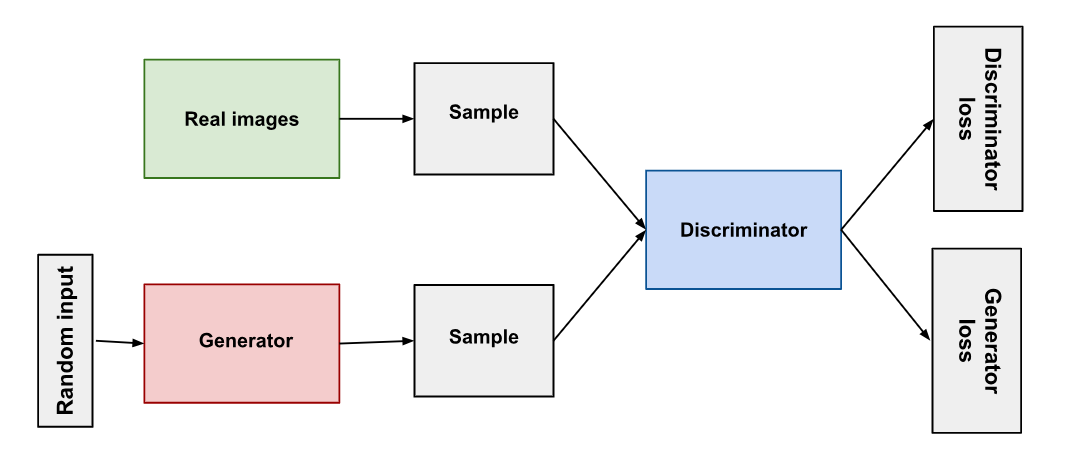
\includegraphics[scale=0.3]{gan}
	\caption{GAN Architecture by Google Developers.}
	\label{fig:gan}
\end{figure}

Convolutional Neural Networks (CNNs) are a class of deep neural networks ideal for tasks such as image analysis and computer vision due to their ability to exploit spatial patterns. Convolutional layers, for which the models are named, slide small filters called kernels over an input, and apply a function which returns one value for the relevant pixels (Figure \ref{fig:cnn}) \cite{cnn}. The result is an output feature map that captures patterns and features of the input image. By changing the kernel, convolutional layers can extract different features of the input.

\begin{figure}[h]
	\centering
        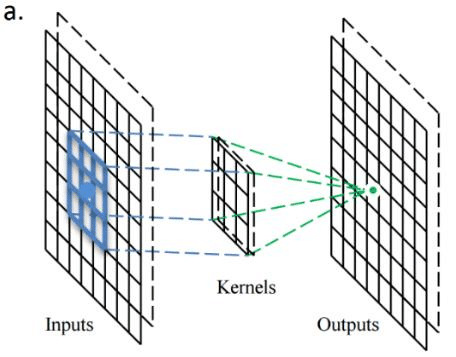
\includegraphics[scale=0.3]{cnn-kernel}
	\caption{Illustration of a convolution kernel.}
	\label{fig:cnn}
\end{figure}

Encoding is the dimensionality reduction of an input image into a lower-dimension feature space representation. For I2I, encoding can be a critical step in extracting relevant and meaningful features from the source images. Likewise, decoding is the reverse process of transforming an encoded representation into a higher-dimensionality output image in the target domain. Both encoding and decoding make use of convolutional layers to change the spatial dimensions of the data.

UNets evolved from CNNs and are often used as the generator in GANs \cite{unet}. They are constructed from a contracting and an expanding block with skip connections, made from convolutional downsampling and upsampling layers (Figure \ref{fig:unet}). Skip connections allow information from previous layers to avoid further processing and be directly passed to later layers, forming bridges that retain various levels of detail and prevent information loss. Often, skip connections in UNets are implemented using concatenation. The skip connections allow the model to detect features at different resolutions, including global structural relationships as well as pixelwise ones.

\begin{figure}[h]
	\centering
        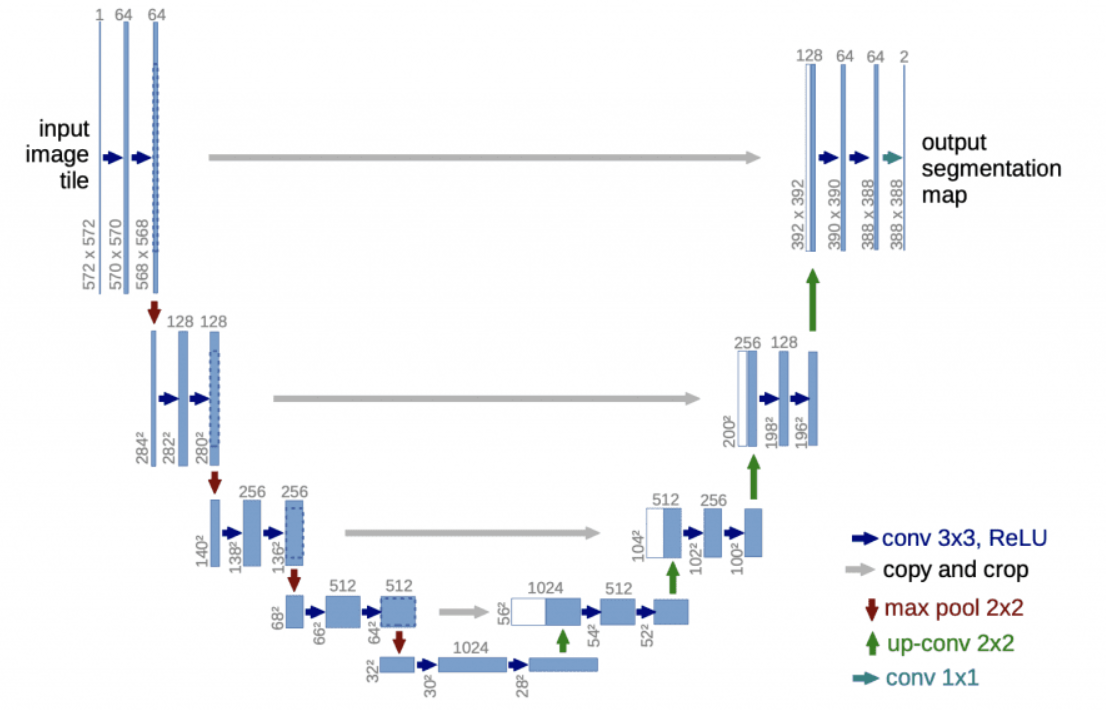
\includegraphics[scale=0.25]{unet}
	\caption{UNet Architecture \cite{unet}.}
	\label{fig:unet}
\end{figure}

Visual transformers (ViTs) are an architecture based off of the Transformer architecture originally designed for language processing. Due to self-attention mechanisms, Transformers are able to capture long-range dependencies in sequential data \cite{transformer}. By applying similar attention mechanisms to image data, ViTs are able to extract relationships between different image features. The general architecture consists of a learnable patch embedding and positional embedding, which create the input vectors to the rest of the ViT. Next, the data goes through alternating layers of multi-head attention and feedforward neural networks before being output \cite{vit}. 

A pixelwise ViT consists of a stack of Transformer encoder blocks \cite{bert}. In the context of image processing, this transformative approach involves representing an image as a sequence of tokens. The series of tokens is formed by flattening the encoded image data. This tokenization process allows the model to represent the image content similarly to text sequences, allowing for the application of the Transformer architecture \cite{bert}. The tokens are then combined with their positional embedding and passed through a feedforward network to enhance the feature representations. Positional embeddings serve as a means to embed the spatial relationships of the tokens, providing the model with an understanding of the original pixel locations within the image.

Recent work has shown that ViTs rival or exceed the capabilities of traditional CNNs \cite{vitcnn}.

All of the aforementioned ML techniques rely on training using loss functions. Loss functions play a crucial role in training a machine learning model by quantifying the difference between the predicted output and the actual ground truth. The design of a loss function significantly impacts the model's ability to learn and generalize effectively by influencing what patterns and features the model prioritizes during training.

The primary goal during training is to minimize the discrepancy between the model's predictions and the true values. The loss function serves as a quantitative measure of this error by providing a clear objective for the model to minimize. The optimization process adjusts the model parameters to achieve this minimization. A good loss function contributes to the model's ability to generalize to unseen data. It encourages the learning of patterns that are representative of the dataset.

Each of these architectures can be used in whole, or in combination with others, to help solve various tasks in machine learning such as I2I. Combining different machine learning architectures can offer several benefits that leverage the strengths of each model. Since each architecture excels at capturing specific features or patterns in data, combining them allows for the extraction of complementary information, potentially enhancing the model's overall representational power. 

Certain architectures may also be well-suited for specific tasks. By combining them, the model can adapt to different aspects of a task, providing a more effective approach to problem-solving. For example, GANs are known for their generative capabilities, while CNNs excel at extracting hierarchical features from input data \cite{ensemble}. Combining GANs with discriminative models like CNNs provides a framework for tasks where both generative and discriminative aspects are crucial, such as for I2I. \cite{cnn} \cite{i2i}

Vision transformers also incorporate attention mechanisms for capturing long-range dependencies. CNN-based UNets perform well at capturing spatial details. Combining the two architectures can allow for more effective attention mechanisms that consider both pixelwise and global relationships. \cite{uvcgan} \cite{vit}

For example, hybrid UNet-GANs \cite{hybrid1}, GANs with ViTs as the discriminator \cite{hybrid2}, and models using an ensemble of CNNs to enrich input to a ViT generator \cite{hybrid3} have all been developed in recent years to great success in classification and image generation tasks. Similarly to these models, the UVCGAN architecture combines CNN encoding and decoding blocks in the format of a UNet, with a vision transformer at the bottleneck of the U. However, combining architectures requires careful design, training, and experimentation to suit the specific requirements of a task. 

\section{Prior Work}

UVCGAN is a deep learning architecture that uses a GAN structure for unpaired image-to-image translation tasks. It revisits the older CycleGAN architecture, the key innovation of which is cycle consistency. This means it trains two generator-discriminator sets: one that transforms images from the source to target domain and one that works in the reverse direction. CycleGAN can learn transformations from unpaired data, making it useful in scenarios where obtaining data pairs is difficult. While this is most beneficial for unpaired image-to-image translation, it is highly versatile and is still a useful tool for paired translation tasks. 

Cycle-consistency loss, a key component of CycleGAN, enforces that the translation from one domain to another and back should bring the image back to the original. This constraint helps improve the quality of generated images and ensures that the learned mappings are coherent and interpretable. \cite{uvcgan}

The UVCGAN generator is a UNet-ViT generator, which is composed of a UNet \cite{unet} with a pixelwise Vision Transformer module at the bottleneck between the encoding and decoding sections \cite{uvcgan}. The UNet consists of four convolutional layers that extract features from inputs by downsampling them. At each downsampling block, a tensor will have its feature dimensions doubled while its width and height are halved. 

The extracted data at each layer are also passed across the net to the matching layers in the decoder through skip connections. At the bottleneck, the data is flattened and passed through the ViT. The architecture uses 12 Transform encoder blocks within the ViT unit, with 384 channel features for input to the ViT. Afterwards, the data is projected and unflattened to original input dimensions. It is then decoded via decoder blocks corresponding to the encoder blocks, and upsampled to create the output image.

\begin{figure}[h]
	\centering
        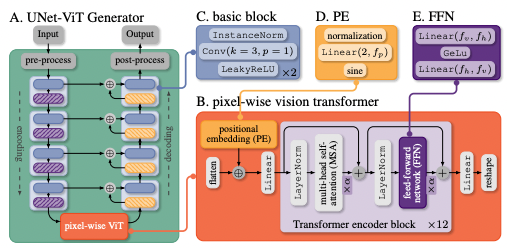
\includegraphics[scale=0.46]{uvcgan}
	\caption{UVCGAN Architecture \cite{uvcgan}.}
	\label{fig:uvcgan}
\end{figure}

While it offers the option to perform paired image translation, UVCGAN has been applied to mainly unpaired domain transformation tasks such as style transfer and response prediction \cite{uvcgan4slats}. I would also like to test its paired transformation capabilities on a task that it has not previously been tested on.

UVCGAN is the architecture I will test and expand on for the task of image denoising.

\section{Methods}

UVCGAN has shown state-of-the-art results in image-to-image translation tasks \cite{uvcgan}. However, I hypothesized that utilizing additional metadata may be helpful for image denoising, where input images all include general image data such as camera type, ISO, and shutter speed. In this project, I will generalize the UVCGAN architecture to include additional modalities and compare its performance to that of the original. In order to store my data and files and train my model, I utilized the GPU partitions of Oxy’s HPC server Bletchley \cite{bletchley}.

My first step was to find and download a suitable dataset, then create a custom dataloader for the images and extract important metadata. I used the small sRGB Smartphone Image Denoising Dataset (SIDD) \cite{sidd}, containing noisy images shot from five different types of smartphone cameras along with clean ground truth images. These images also come with shooting data such as smartphone camera type, ISO, shutter speed, temperature, and brightness. 

I chose a smartphone image dataset because the majority of people take photos on their smartphones; additionally, smartphone cameras tend to prioritize size over quality, so smartphone cameras are more likely to produce lower quality images that require denoising \cite{cam}. For everyday purposes, denoising is likely not necessary; however, there may be special cases for aesthetic or security considerations where noise removal is desired. 

I wrote a script to restructure the dataset, then began writing a custom dataloader extending a PyTorch DataLoader. Because this project is a proof of concept and the original architecture is already very large, in order to reduce training time and resource usage, I cropped each image to 256x256 pixels. Ideally, full size images would be used.

I also created a multimodal modification of my dataloader, where the image would be returned along with the metadata extracted from it, including ISO, shutter speed, and temperature.

Once I had the dataset and dataloader set up, I then attempted to create my own training script for the model in order to better understand the necessary steps to train a model. I also thought it would be easier to perform my architecture modifications that way. Unfortunately, when I tested the training script on the existing architecture, I discovered that all the pixel values rapidly approached red (255, 0, 0) for color images and black (0.0) for grayscale images. I spent around 20 hours going through the code, debugging, testing, and meeting with various professors to try and find out what was going wrong. Despite all that effort, I was still unable to find out why the model was behaving that way, which forced me to scrap my custom training script and instead modify the example training scripts provided by the developers for style transfer tasks. 

After I successfully created new training scripts, I ran baseline tests using both L1 (Mean Absolute Error) and L2 (Mean Squared Error) loss functions (see Metrics section for more details), 120 epochs, and batch size 4. 

My hyperparameter selections and the reasoning are as follows. I ran 120 epochs because I was limited to a maximum allowed effective runtime of around 140 epochs on the HPC server. In addition, preliminary tests showed that the loss began to flatten out around 80 epochs. Batch size was 4 because I was only able to access the small version of the dataset, and I wanted to train through many batches in each iteration. The optimizer, scheduler, and their hyperparameters were left as model default presets, which were AdamW and CosineAnnealingWarmRestarts respectively.

\begin{figure}[h]
	\centering
        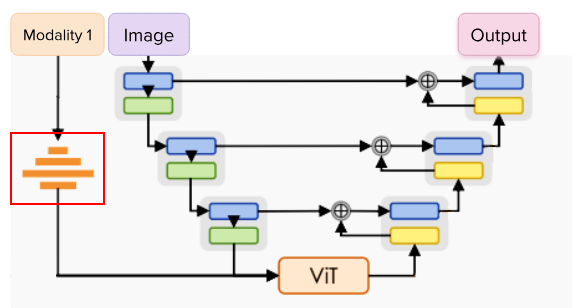
\includegraphics[scale=0.41]{images/mm_arch.png}
	\caption{Overall diagram of the multimodal modification of UVCGAN. Small network upsampling metadata is highlighted by the red box and is shown in greater detail in (Figure \ref{fig:smallnetwork}).}
	\label{fig:mm_arch}
\end{figure}

\begin{figure}[h]
	\centering
        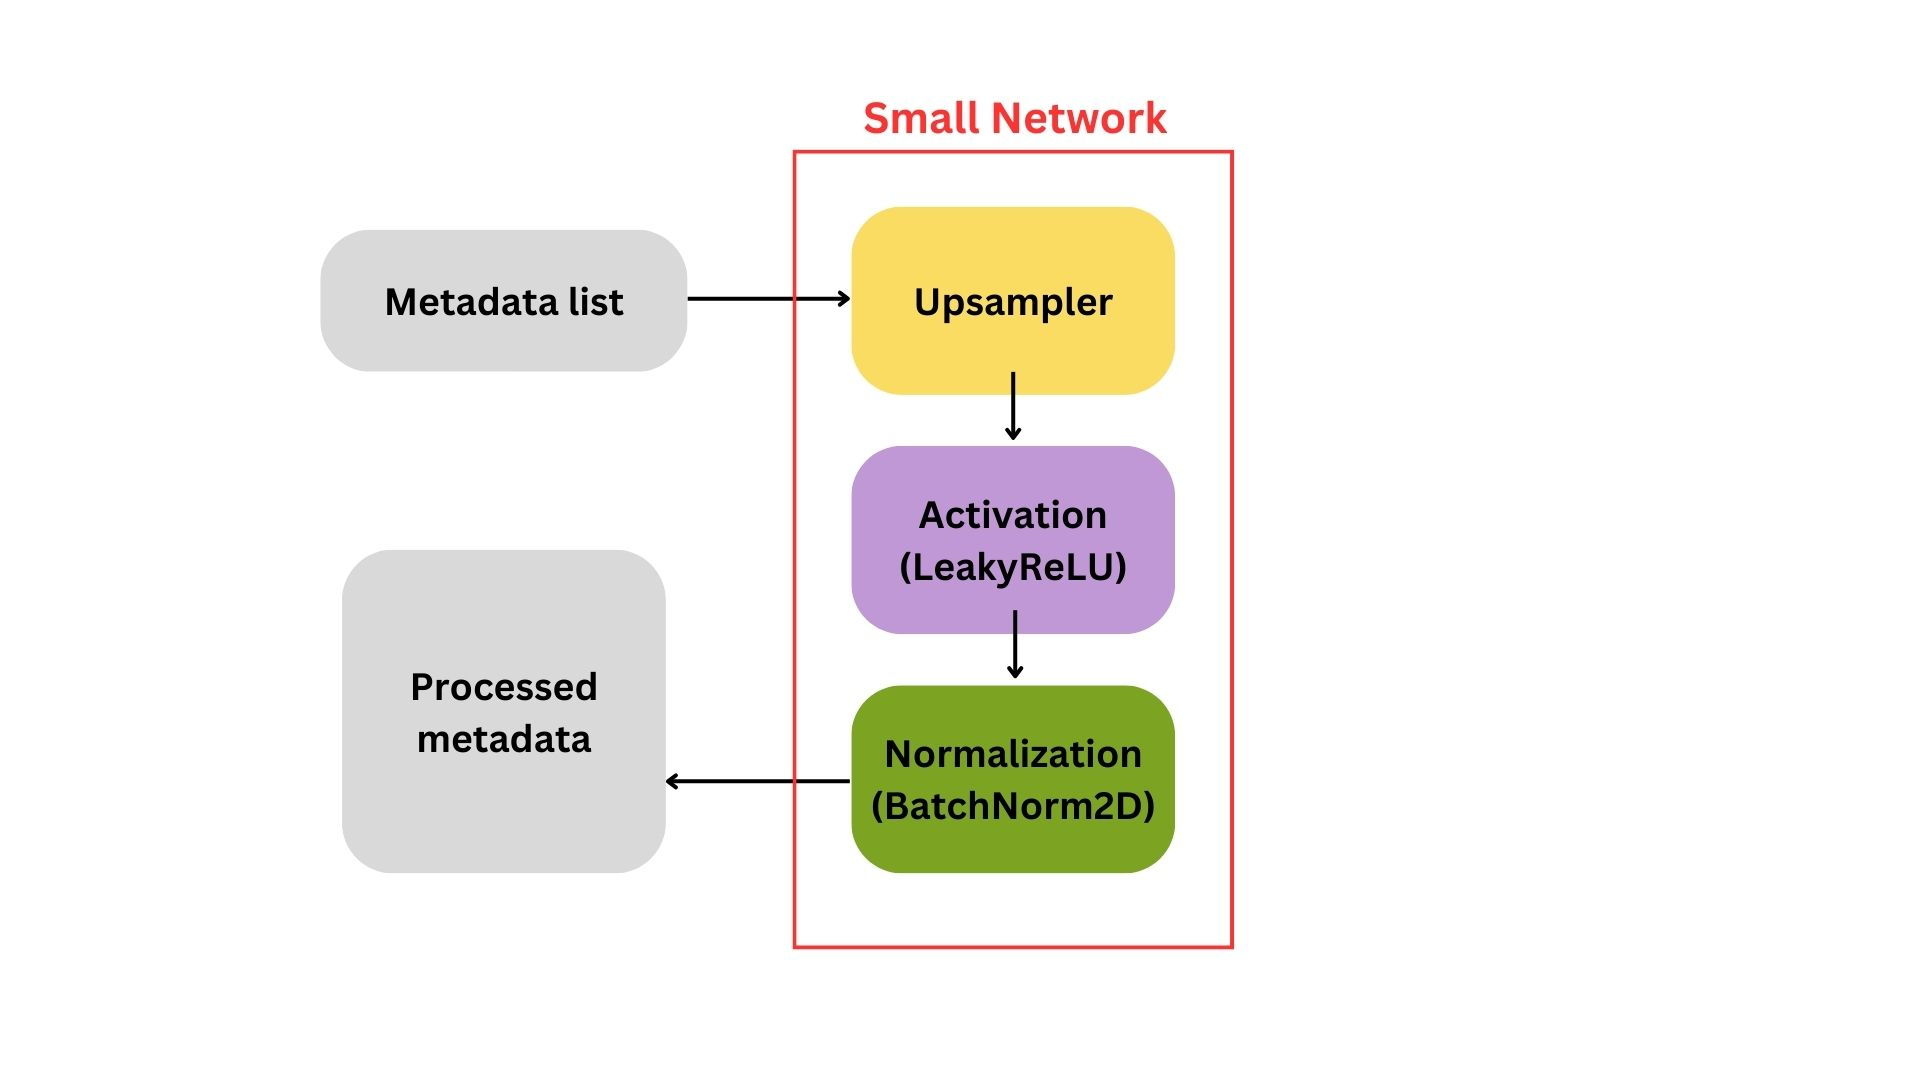
\includegraphics[scale=0.2]{images/smallnetwork.jpg}
	\caption{Components of the small network that processes the camera metadata.}
	\label{fig:smallnetwork}
\end{figure}

Then, I created the multimodal version of the UVCGAN architecture. 
To do this, I first created a feedforward network to pass the provided metadata into. It took in an input array of dimension 1 with length equal to the number of unique metadata parameters considered, upsampled it to the size of the channel where it would be concatenated later, then passed through an activation and normalization layer (Figure \ref{fig:smallnetwork}). The size of the channel is passed in during model initialization, rather than hardcoded, so it is adaptable to any size dimensions.

The processed metadata is concatenated only at the very bottom of the encoding section, immediately before the combined data is passed into the vision transformer (Figure \ref{fig:mm_arch}). In both my version and the original architecture, the Vision Transformer takes an input with 384 features. This means that for the last encoding block, instead of upsampling to 384 features, I upsample to 383 features, leaving one feature channel for the processed camera metadata which has the same width and height dimensions.

However, the metadata has to be passed in through the top of the encoder block at the initialization and calling of the ViT-UNet architecture, and trickled down to the components. The ViT-UNet initializes a UNet, which is composed of UNet Blocks consisting of Encoding and Decoding blocks. The metadata is passed down through the ViTUNet and UNet to the UNet Blocks, where the upsampler and small network are initialized at the bottleneck of the U, between the encoders and decoders (the point where the number of output feature channels is 384). It is passed through the small network and concatenated to the rest of the encoded image data before being passed into the ViT.

My reasoning for this method of modality combination was that since the metadata is not part of the pixel image data, it does not make sense to concatenate it early on and encode it as if it were part of the image. It also is more reasonable to train a separate small network on how to represent the metadata post-upsampling, since it should be treated separately from the image data. In addition, it seemed more sensible to concatenate the metadata as an additional channel to the image data, rather than add it to the RGB pixel values in each channel of the image data, for the same reasons.

After debugging and short test runs, I ran the multimodal model with the same parameter variations as for the baseline. For each, training took around 4 hours for both multimodal and baseline models. After training each model, I generated images using a test set to represent the performance of the model on previously unseen data, to evaluate how well it had learned the relationships between noisy and clean images.

I then conducted qualitative and quantitative analyses of the results, using the output generated images and loss metrics respectively (discussed further in Metrics/Evaluation and Results/Discussion sections).

\section{Metrics and Evaluation}

For my project, quantitative metrics are the losses, and my overall project evaluation is linked to, but separate from, the quantitative performance because it is an experiment of a new architecture.

The two metrics I used to train my models were L1 and L2. These are two common losses that can be leveraged for deep neural nets such as UVCGAN.

L1 loss, Mean Absolute Error, is calculated by averaging the differences between the predictions and targets over the batch or dataset. It helps to ensure sparseness of representations, which means that only a fraction of the elements in a representation or activation vector are non-zero. Sparsity is desirable because it increases the resource and computational efficiency of the model, while also acting as a form of regularization by forcing the model to focus on a small subset of features \cite{janochaloss}.

L2, or Mean Squared Error, is the most commonly used loss function for machine learning. It is a simple function that squares the L1 loss and averages it across the batch or dataset. Because the differences are squared, it penalizes outliers more heavily than L1, which can be desirable depending on the specific use case. Additionally, the L2 curve is differentiable everywhere, which simplifies the optimization process by allowing for use of optimization algorithms that use gradient calculations such as Stochastic Gradient Descent \cite{janochaloss}. 

Even though the L2 loss has several advantages over L1 in terms of optimization, L1 has been shown to perform better for image reconstruction tasks \cite{lossblur} (See Results and Discussion for further discussion).

In my project, I trained the model and my modifications using both of these loss functions to compare their performance. Reasonable loss vs epoch curves are a sign that my model is training properly, and point towards a successful project.

To evaluate the success of my project as a whole, I have set the following objectives and evaluation methods: 

\begin{enumerate}
  \item Gain a deep understanding of the ViT-UNet architecture, the success of which will be evaluated by my ability to inject an additional modality into the architecture. 
  \begin{enumerate}
        \item The accuracy/performance of this modification should be reasonable, but this objective will not be evaluated solely based on how well the architecture performs on the given task.
  \end{enumerate}
  \item Explore how different loss functions, specifically L1 and L2, impact the model’s training and its image reconstruction performance. 
  \begin{enumerate}
      \item For this objective, I expect to be able to use characteristics of each loss function to explain variation between the results for models trained on each, as well as an overall evaluation of which performs better and where it may still be lacking. 
  \end{enumerate}
\end{enumerate}

\section{Results and Discussion}

\begin{figure*}
  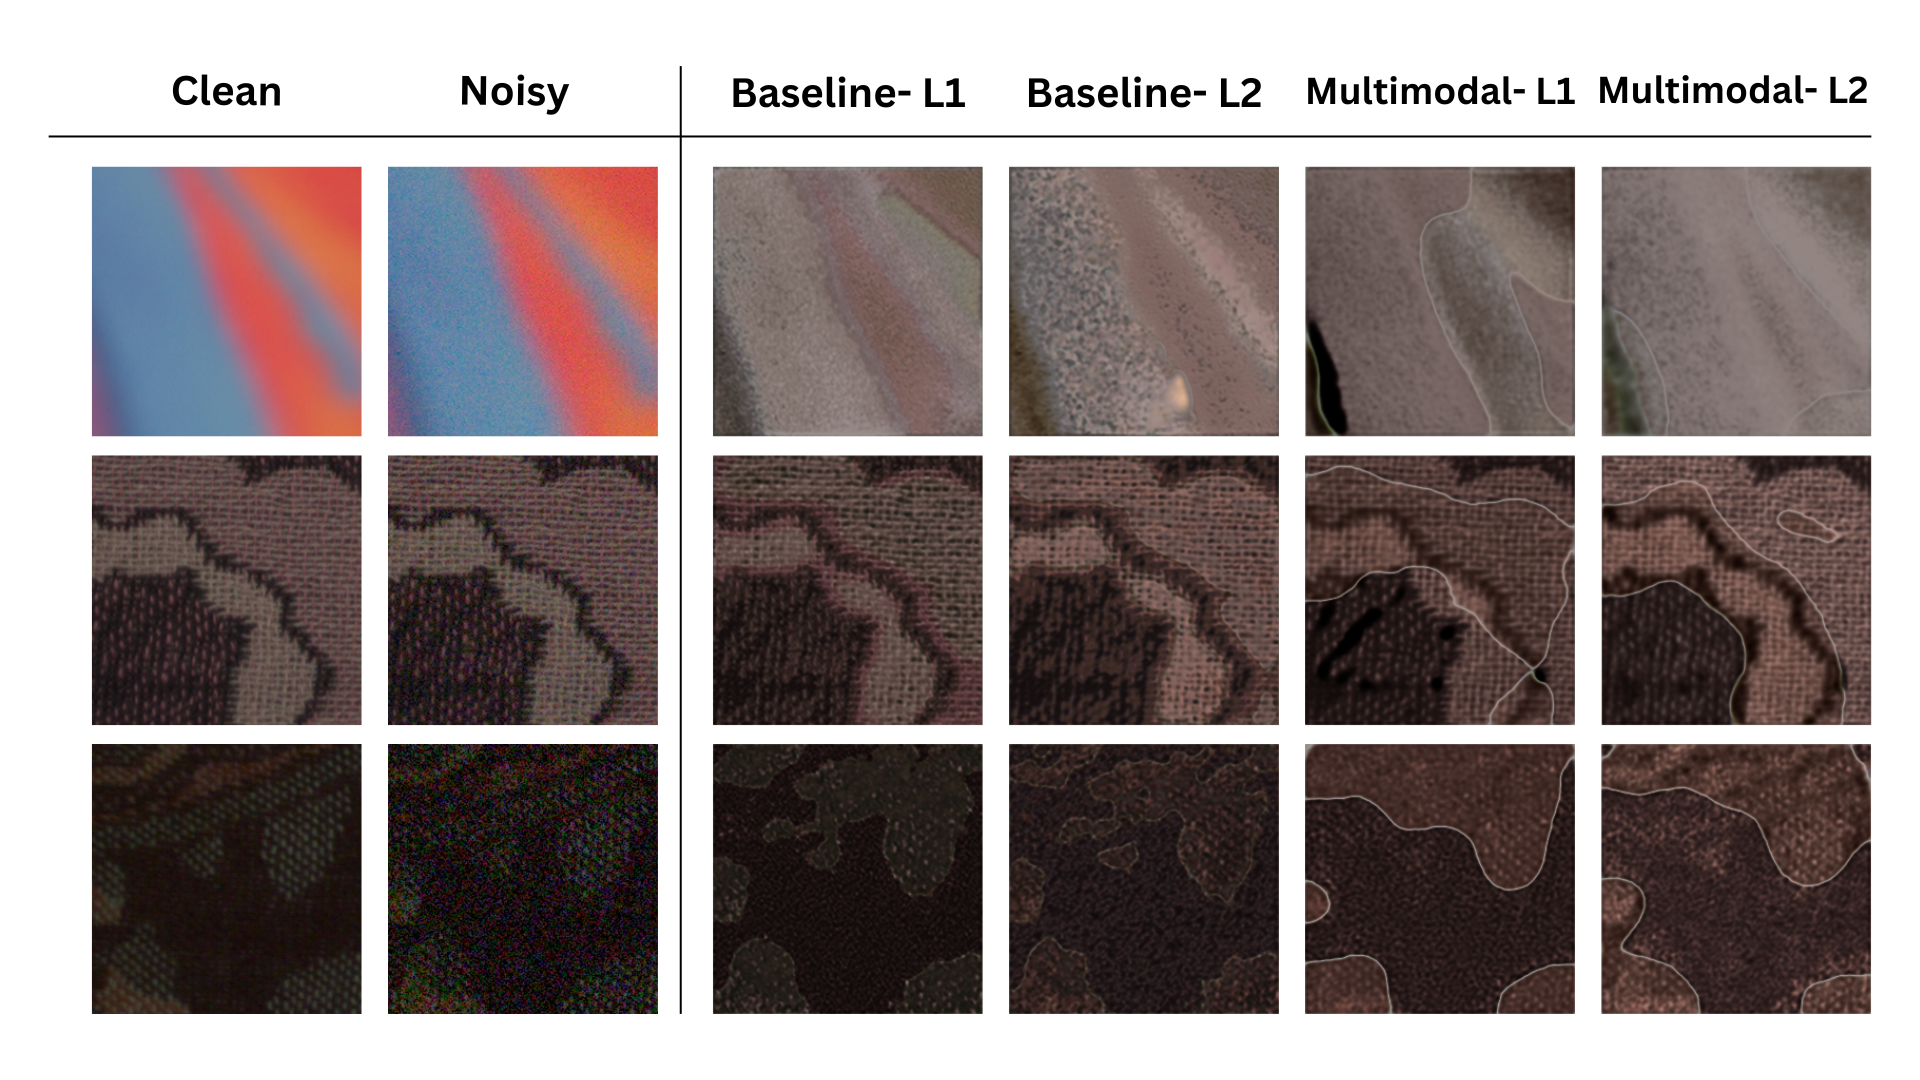
\includegraphics[width=\textwidth]{images/table.png}
  \caption{Image generation results for baseline and multimodal runs with L1 and L2 loss, along with input (noisy) and target (ground truth) images.}
  \label{fig:table}
\end{figure*}

I found that this model, run with the hyperparameters and loss functions that I stated previously, is capable of removing color noise from images, but usually does not create satisfactory image reconstructions. This suggests that hyperparameter tuning is needed to improve the model performance. However, if hyperparameter tuning is still unable to produce improved results, the architecture simply may not be well suited for image denoising.

A qualitative analysis of the generated results (Figure \ref{fig:table}) shows that L1 loss produced higher fidelity image reconstructions than L2 in both my baseline and experimental runs. This supports evidence in previous work that L1 produces more realistic images than L2 loss. Both L1 and L2 loss are known to produce slightly blurry image reconstructions \cite{lossblur}, but L1 generally produces less blur than L2 due to L2’s tendency to over-smooth \cite{lossdocs}.

However, while the models were successful in removing noise, both loss functions produced images with poor color recall [FIGURE]. Additionally, the multimodal architecture produced images with gray outlines around regions of different colors or significantly differing amounts of noise. Baseline L2 runs also produced these lines, but to a lesser extent.

\begin{figure}[h]
	\centering
        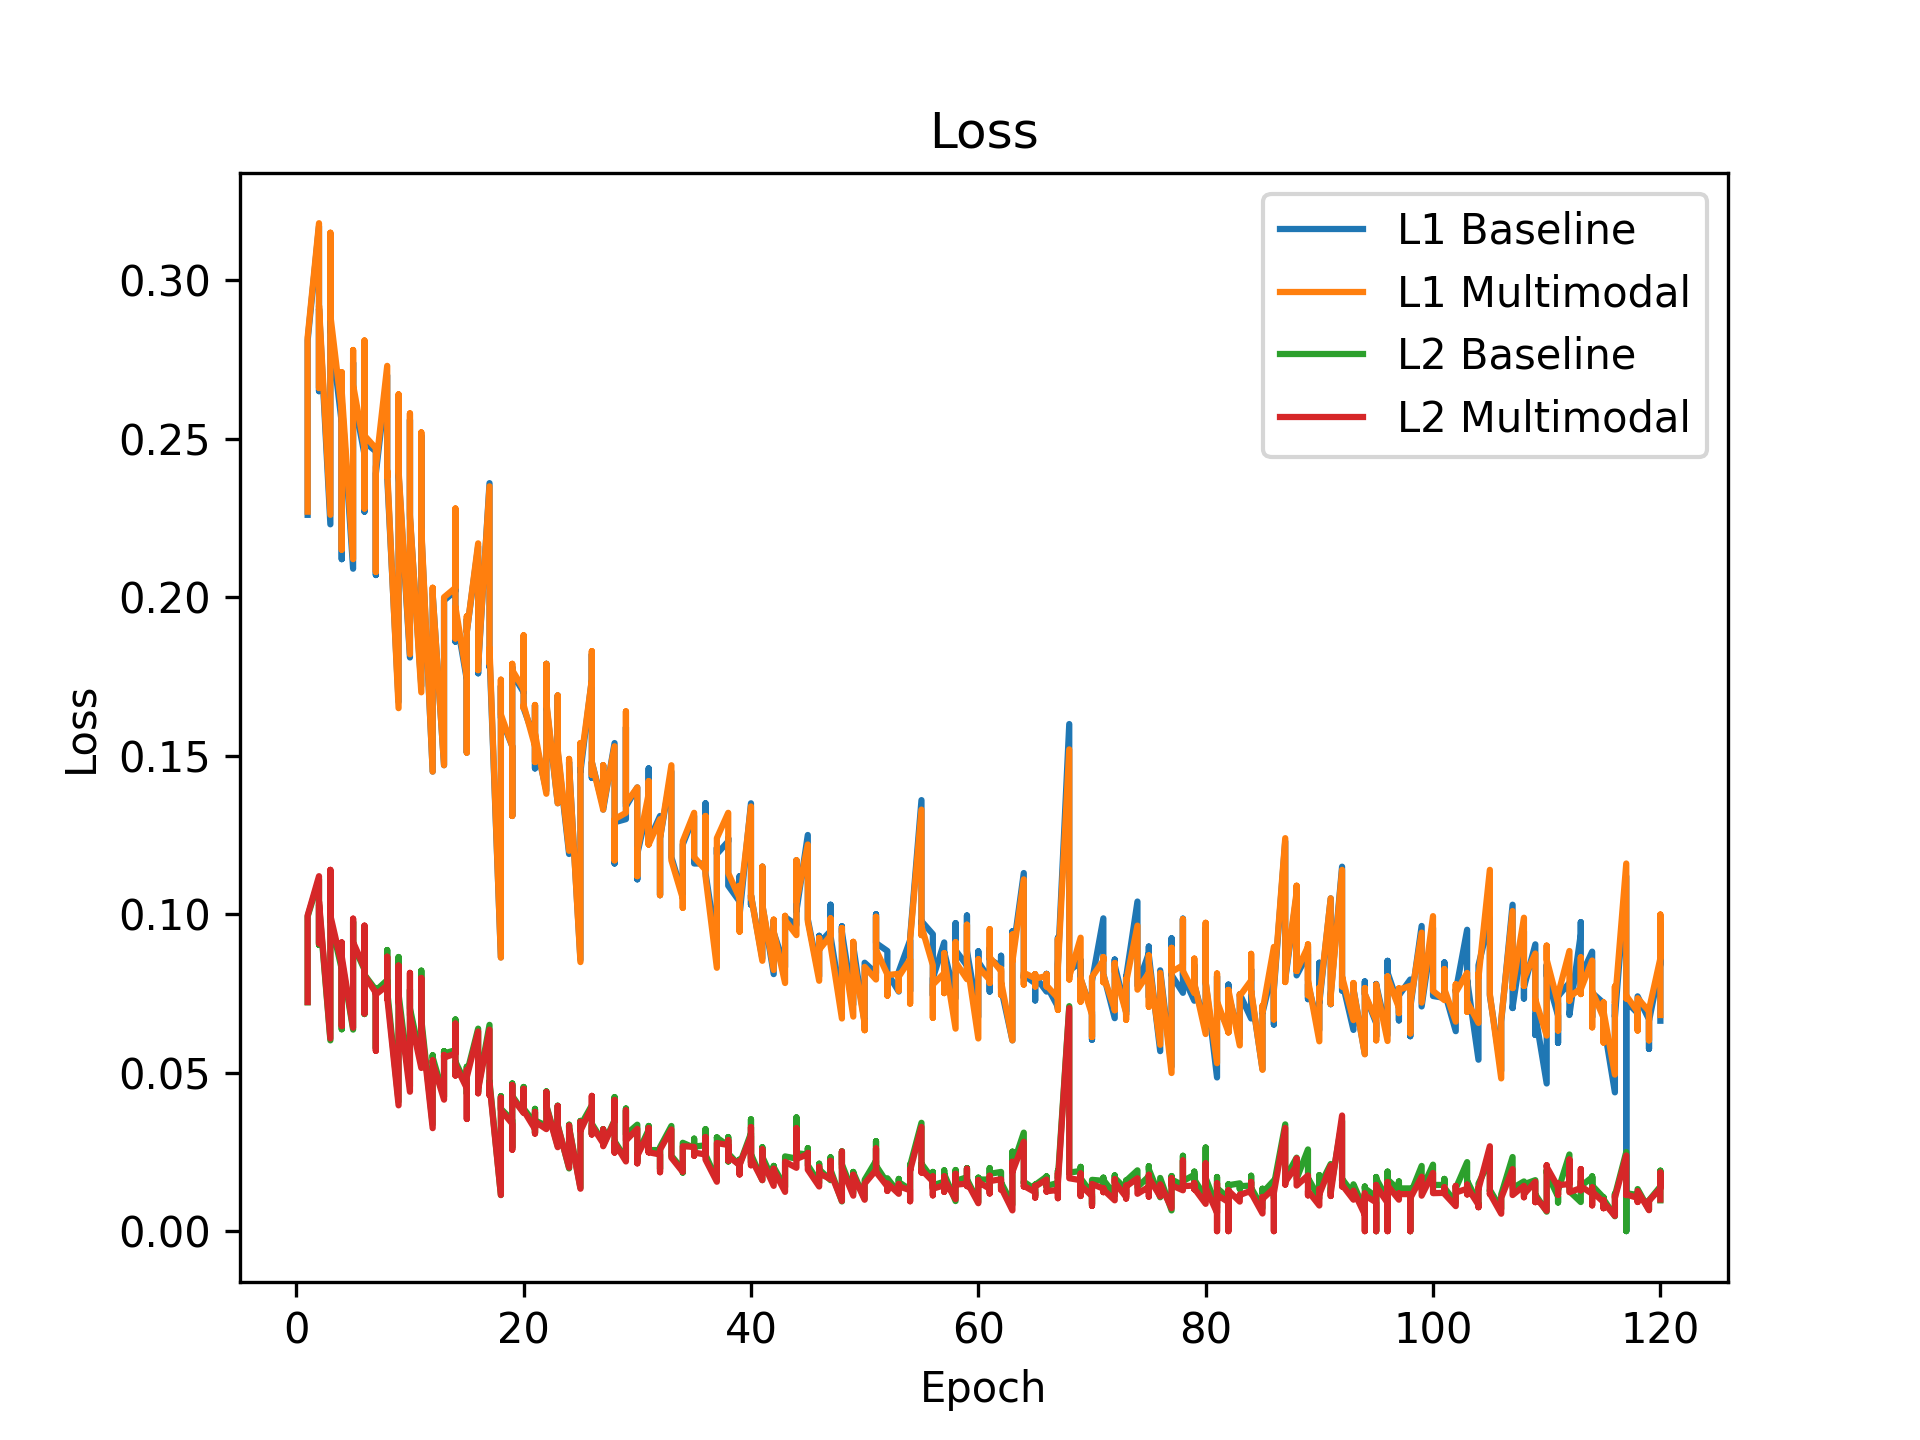
\includegraphics[scale=0.5]{images/lossplot.png}
	\caption{Loss plot for all four experimental runs.}
	\label{fig:lossplot}
\end{figure}

The loss curves for the multimodal and original versions of UVCGAN with L1 loss flatten out at the same point; similar variance remains in the loss for the multimodal architecture compared to the original after this point is reached, at roughly 75 training epochs (Figure \ref{fig:lossplot}). 

After a qualitative analysis of the generated images, I noticed that while some noise was removed, and nearly all the color noise was removed successfully, images with color did not retain their vibrancy in the reconstructions. This suggested that the loss functions used were not ideal for training. 

At the poster presentations, Professors Vo and Leonard both suggested the same observation as feedback. I investigated common loss functions used for image reconstruction and found that after L1 and L2, SSIM (structural similarity) was the most commonly used function. At the beginning of the project, I had intended to use a custom loss function consisting of a combination of L1 and SSIM, which has been shown to have higher performance than both L1, SSIM, and L2 alone \cite{L1ssim}. However, I had to translate the function from Caffe to PyTorch, and ran into issues with debugging. After my test runs, I noticed my images preserved global image structure very well, so I decided a loss function that weighted global structure even more heavily was unnecessary. As a result I did not end up completing the translation and implementing the L1-SSIM loss function. 

Based on the professors' feedback I considered several possible alternatives to weight color retention more heavily, but decided ultimately to prioritize completing the multimodal implementation due to time constraints.

As a whole, I believe that I accomplished both of my project goals. I successfully modified the architecture to inject an additional modality. The multimodal architecture’s performance was worse than that of the original, which suggests that many further modifications and testing are needed. In particular, the small network upsampling the metadata should be changed as this is just one of countless different possible methods to represent the metadata. Changes to this small network will be relatively simple in terms of organization because it is contained entirely in one file. Unfortunately, I did not have time to test many different small network architectures; perhaps this is the next step for future work extending this project.

\section{Ethical Considerations}

\subsection{Topic Overview}
My project explores the efficacy of a multimodal ViT-UNet framework for image denoising. As is the case with all applications of technology to solve problems, there are ethics issues that must be taken into consideration. While it may be impossible to completely mitigate all ethical problems that come up, recognizing them is the first step to doing what one can to solve them.

\subsection{Implicit Bias}
In all areas of life, including research that seeks to uncover truth or knowledge, it is impossible to avoid implicit bias. Humans are naturally predisposed to certain beliefs and preferences, and it is important to recognize these biases in others', as well as one's own, work. 

In this project I apply my model to a broad variety of images. My goal is to use as diverse a set of data as possible, but there are some limitations. I will be working with multimodal data; this means that I will be using images that contain metadata such as utilized here. Therefore, users who only have access to a camera that does not store such data may not directly benefit from my project. Since these cameras are likely to be cheaper to purchase, especially compared to smartphones, and not require photography knowledge, my project may disproportionately benefit certain demographics more than others. At the same time, the quality of the photos that the majority of people are able to capture without further processing is at an acceptable level for their needs. Many would not think of the processing time required to feed thousands of their photos through a denoising algorithm as worth the slight increase in photo quality.

Given a user base of smartphone as well as DSLR camera owners, my project attempts to remove some of the photo quality discrepancies caused by the difference in equipment price and quality. For example, a student photographer should not have to purchase a camera in the range of thousands of dollars to get a decent night exposure photo. My project also aims to help remove some of the glaring photo quality issues that often arise with high ISO and long exposures, so that users with more affordable cameras or only access to smartphone cameras can still capture scenes with those camera settings.

\subsection{Privacy and Consent}
I am using publicly available, and widely benchmarked, photo datasets. SIDD (Smartphone Image Denoising Dataset) is a dataset containing thousands of noisy images from five different types of real smartphone cameras under different lighting conditions, with corresponding clean ground truth images \cite{sidd}.

No personal data has been collected or handled. I do not anticipate any privacy and consent issues with the data I used in this project.

\subsection{Potential for Abuse}
As with any algorithm, there is the risk of it being used for malicious purposes. Image manipulation in particular can be used to spread false information. Often, forged images have distinct patterns of noise that are key to the identification of fake images. However, denoising algorithms can be used to remove this noise and make fake images more realistic.

Exposure manipulation and denoising may allow people to violate others’ privacy, by taking advantage of the model’s capabilities to see things that normally would have been hidden by the dark or by low surveillance camera quality.

In addition, the use of denoising algorithms to remove watermarks can be used to violate copyright laws and enable its distribution \cite{watermark}.

Unfortunately, it is often difficult or impossible to control how others will misuse an algorithm. I plan to use it with the best intentions to increase accessibility, but it may well be used with malicious intent as well if it falls in the wrong hands. This is, however, more of a societal issue than any that can be solved with technology alone. 

\subsection{Technological Solutionism}

Oftentimes, applications of machine learning to solve real-world problems can be reduced to a form of technological solutionism where people treat ML and AI as a blackbox that can just solve a problem. However, this is a dangerous way of thinking as it disregards many safety and ethical principles, sets false promises, and further perpetuates an unrealistic view of ML and AI \cite{ts}. Additionally, defaulting to new technology to solve problems only reinforces economic, resource, and class inequalities in society. As such, we should first seek to find societal and non-technological solutions to the root of a problem instead of using technology to disguise it.

However, in this case, technology is one of the best solutions to increasing instant accessibility to high-quality image capture technology. Because camera sensors and lenses are intrinsically expensive and difficult to make, high-quality photography especially in low light conditions can be a very expensive goal. In the past, photographers and researchers would have no other option but to save their money for better imaging equipment. The typical beginner photographer or smartphone owner is unable to afford this cost. However, a deep learning algorithm can potentially provide a quick, easy way to enhance image quality without needing to pay for sensors that can capture an equivalent image as is. 

Overall, I believe the benefits of my project that can be used to increase accessibility outweigh the reasonable ethics and misuse concerns. 

\section{Future Work}

There is much future work that can be done in this project. The model's poor performance on image denoising suggests that hyperparameter tuning is needed, along with modifications to the small network used to upsample and process camera metadata. An investigation into the segmentation artifacts generated by the multimodal model may also be of interest.

Additionally, the computational resources needed to train this model are significant. Without a HPC resource or GPU, it would be very difficult to train. An optimization of the architecture to increase resource and time efficiency would be helpful for anyone who would like to run this code in the future.

A larger extension of the project lies in video footage editing. The proven style transfer capabilities of UVCGAN \cite{uvcgan} can potentially be adapted to video frames to transform footage.

\section{Conclusions}

This project explored the use of an existing I2I architecture for the task of image denoising, and provided a proof of concept for a multimodal version of the architecture. It was tested using different smartphone images and lens types, but is easily extendable to any situation where additional shooting data is available. However, for the multimodal modification, much further work also needs to be done to boost performance and create a model suitable for real life use. Further experimentation and testing can help determine which tasks it may be best suited for, and how to adapt it to different I2I tasks.

Overall, I gained a deep understanding of many machine learning techniques such as GANs, CNNs, UNets, and specific loss functions. By modifying the code that makes up such architectures, I was able to practice actual implementation, going beyond the conceptual level that my courses had taught me about them.

\footnote{Link to Overleaf project: \url{https://www.overleaf.com/read/ybgxypcphwkt}}


\printbibliography

\end{document}
